% ==============================================================
% --- Git
% ==============================================================
\section{Automated Version Control}\hypertarget{sec1}{}

\begin{frame}[fragile]
\frametitle{Why version control?}

  \begin{columns}

    \begin{column}{0.6\textwidth}
      Problems
      \begin{itemize}
        \small
        \item Multiple, nearly identical versions of the same document
        \item Tracking changes is not an option for source code
        \item No protection against accidental deletion
      \end{itemize}
      \vspace{0.15cm}
      Version control systems 
      \begin{itemize}
        \small
        \item {\bf start} with a base version of the document
        \item {\bf record} changes you make each step of the way
        \item can {\bf revert} to any previous versions if necessary
        \item {\bf never lose} a previous state of your document
        \item allow many people to {\bf work in parallel}
      \end{itemize}
    \end{column}

    \begin{column}{0.4\textwidth}
    \begin{figure}[h]
    
\includegraphics[width=0.9\textwidth]{sec1/comic_version_control.png}
    \end{figure}
    \end{column}

  \end{columns}

\end{frame}

\begin{frame}[fragile]
\emptyframetitle
  \begin{columns}
    \begin{column}{0.33\textwidth}
{\bf Sequential changes}
      \begin{figure}[h]
      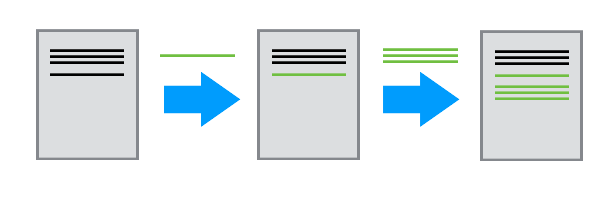
\includegraphics[width=1.0\textwidth]{sec1/change.png}
      \end{figure}
      Start at the base document, apply each change, arrive at the more recent version
    \end{column}
    \begin{column}{0.33\textwidth}
{\bf Diverging versions}
      \begin{figure}[h]
      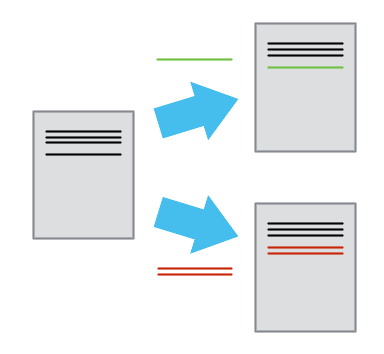
\includegraphics[width=1.0\textwidth]{sec1/versions.png}
      \end{figure}
      Two users can make independent sets of changes on the same document
    \end{column}
    \begin{column}{0.33\textwidth}
{\bf Merge versions}
      \begin{figure}[h]
      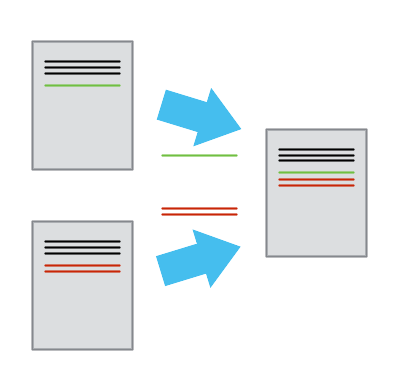
\includegraphics[width=1.0\textwidth]{sec1/merge.png}
      \end{figure}
      Incorporate two sets of changes into the same base document
    \end{column}

  \end{columns}

\end{frame}
